% Options for packages loaded elsewhere
\PassOptionsToPackage{unicode}{hyperref}
\PassOptionsToPackage{hyphens}{url}
\PassOptionsToPackage{dvipsnames,svgnames,x11names}{xcolor}
%
\documentclass[
  a4paperpaper,
  DIV=11,
  numbers=noendperiod]{scrartcl}

\usepackage{amsmath,amssymb}
\usepackage{iftex}
\ifPDFTeX
  \usepackage[T1]{fontenc}
  \usepackage[utf8]{inputenc}
  \usepackage{textcomp} % provide euro and other symbols
\else % if luatex or xetex
  \usepackage{unicode-math}
  \defaultfontfeatures{Scale=MatchLowercase}
  \defaultfontfeatures[\rmfamily]{Ligatures=TeX,Scale=1}
\fi
\usepackage{lmodern}
\ifPDFTeX\else  
    % xetex/luatex font selection
\fi
% Use upquote if available, for straight quotes in verbatim environments
\IfFileExists{upquote.sty}{\usepackage{upquote}}{}
\IfFileExists{microtype.sty}{% use microtype if available
  \usepackage[]{microtype}
  \UseMicrotypeSet[protrusion]{basicmath} % disable protrusion for tt fonts
}{}
\makeatletter
\@ifundefined{KOMAClassName}{% if non-KOMA class
  \IfFileExists{parskip.sty}{%
    \usepackage{parskip}
  }{% else
    \setlength{\parindent}{0pt}
    \setlength{\parskip}{6pt plus 2pt minus 1pt}}
}{% if KOMA class
  \KOMAoptions{parskip=half}}
\makeatother
\usepackage{xcolor}
\setlength{\emergencystretch}{3em} % prevent overfull lines
\setcounter{secnumdepth}{-\maxdimen} % remove section numbering
% Make \paragraph and \subparagraph free-standing
\ifx\paragraph\undefined\else
  \let\oldparagraph\paragraph
  \renewcommand{\paragraph}[1]{\oldparagraph{#1}\mbox{}}
\fi
\ifx\subparagraph\undefined\else
  \let\oldsubparagraph\subparagraph
  \renewcommand{\subparagraph}[1]{\oldsubparagraph{#1}\mbox{}}
\fi

\usepackage{color}
\usepackage{fancyvrb}
\newcommand{\VerbBar}{|}
\newcommand{\VERB}{\Verb[commandchars=\\\{\}]}
\DefineVerbatimEnvironment{Highlighting}{Verbatim}{commandchars=\\\{\}}
% Add ',fontsize=\small' for more characters per line
\usepackage{framed}
\definecolor{shadecolor}{RGB}{241,243,245}
\newenvironment{Shaded}{\begin{snugshade}}{\end{snugshade}}
\newcommand{\AlertTok}[1]{\textcolor[rgb]{0.68,0.00,0.00}{#1}}
\newcommand{\AnnotationTok}[1]{\textcolor[rgb]{0.37,0.37,0.37}{#1}}
\newcommand{\AttributeTok}[1]{\textcolor[rgb]{0.40,0.45,0.13}{#1}}
\newcommand{\BaseNTok}[1]{\textcolor[rgb]{0.68,0.00,0.00}{#1}}
\newcommand{\BuiltInTok}[1]{\textcolor[rgb]{0.00,0.23,0.31}{#1}}
\newcommand{\CharTok}[1]{\textcolor[rgb]{0.13,0.47,0.30}{#1}}
\newcommand{\CommentTok}[1]{\textcolor[rgb]{0.37,0.37,0.37}{#1}}
\newcommand{\CommentVarTok}[1]{\textcolor[rgb]{0.37,0.37,0.37}{\textit{#1}}}
\newcommand{\ConstantTok}[1]{\textcolor[rgb]{0.56,0.35,0.01}{#1}}
\newcommand{\ControlFlowTok}[1]{\textcolor[rgb]{0.00,0.23,0.31}{#1}}
\newcommand{\DataTypeTok}[1]{\textcolor[rgb]{0.68,0.00,0.00}{#1}}
\newcommand{\DecValTok}[1]{\textcolor[rgb]{0.68,0.00,0.00}{#1}}
\newcommand{\DocumentationTok}[1]{\textcolor[rgb]{0.37,0.37,0.37}{\textit{#1}}}
\newcommand{\ErrorTok}[1]{\textcolor[rgb]{0.68,0.00,0.00}{#1}}
\newcommand{\ExtensionTok}[1]{\textcolor[rgb]{0.00,0.23,0.31}{#1}}
\newcommand{\FloatTok}[1]{\textcolor[rgb]{0.68,0.00,0.00}{#1}}
\newcommand{\FunctionTok}[1]{\textcolor[rgb]{0.28,0.35,0.67}{#1}}
\newcommand{\ImportTok}[1]{\textcolor[rgb]{0.00,0.46,0.62}{#1}}
\newcommand{\InformationTok}[1]{\textcolor[rgb]{0.37,0.37,0.37}{#1}}
\newcommand{\KeywordTok}[1]{\textcolor[rgb]{0.00,0.23,0.31}{#1}}
\newcommand{\NormalTok}[1]{\textcolor[rgb]{0.00,0.23,0.31}{#1}}
\newcommand{\OperatorTok}[1]{\textcolor[rgb]{0.37,0.37,0.37}{#1}}
\newcommand{\OtherTok}[1]{\textcolor[rgb]{0.00,0.23,0.31}{#1}}
\newcommand{\PreprocessorTok}[1]{\textcolor[rgb]{0.68,0.00,0.00}{#1}}
\newcommand{\RegionMarkerTok}[1]{\textcolor[rgb]{0.00,0.23,0.31}{#1}}
\newcommand{\SpecialCharTok}[1]{\textcolor[rgb]{0.37,0.37,0.37}{#1}}
\newcommand{\SpecialStringTok}[1]{\textcolor[rgb]{0.13,0.47,0.30}{#1}}
\newcommand{\StringTok}[1]{\textcolor[rgb]{0.13,0.47,0.30}{#1}}
\newcommand{\VariableTok}[1]{\textcolor[rgb]{0.07,0.07,0.07}{#1}}
\newcommand{\VerbatimStringTok}[1]{\textcolor[rgb]{0.13,0.47,0.30}{#1}}
\newcommand{\WarningTok}[1]{\textcolor[rgb]{0.37,0.37,0.37}{\textit{#1}}}

\providecommand{\tightlist}{%
  \setlength{\itemsep}{0pt}\setlength{\parskip}{0pt}}\usepackage{longtable,booktabs,array}
\usepackage{calc} % for calculating minipage widths
% Correct order of tables after \paragraph or \subparagraph
\usepackage{etoolbox}
\makeatletter
\patchcmd\longtable{\par}{\if@noskipsec\mbox{}\fi\par}{}{}
\makeatother
% Allow footnotes in longtable head/foot
\IfFileExists{footnotehyper.sty}{\usepackage{footnotehyper}}{\usepackage{footnote}}
\makesavenoteenv{longtable}
\usepackage{graphicx}
\makeatletter
\def\maxwidth{\ifdim\Gin@nat@width>\linewidth\linewidth\else\Gin@nat@width\fi}
\def\maxheight{\ifdim\Gin@nat@height>\textheight\textheight\else\Gin@nat@height\fi}
\makeatother
% Scale images if necessary, so that they will not overflow the page
% margins by default, and it is still possible to overwrite the defaults
% using explicit options in \includegraphics[width, height, ...]{}
\setkeys{Gin}{width=\maxwidth,height=\maxheight,keepaspectratio}
% Set default figure placement to htbp
\makeatletter
\def\fps@figure{htbp}
\makeatother
% definitions for citeproc citations
\NewDocumentCommand\citeproctext{}{}
\NewDocumentCommand\citeproc{mm}{%
  \begingroup\def\citeproctext{#2}\cite{#1}\endgroup}
\makeatletter
 % allow citations to break across lines
 \let\@cite@ofmt\@firstofone
 % avoid brackets around text for \cite:
 \def\@biblabel#1{}
 \def\@cite#1#2{{#1\if@tempswa , #2\fi}}
\makeatother
\newlength{\cslhangindent}
\setlength{\cslhangindent}{1.5em}
\newlength{\csllabelwidth}
\setlength{\csllabelwidth}{3em}
\newenvironment{CSLReferences}[2] % #1 hanging-indent, #2 entry-spacing
 {\begin{list}{}{%
  \setlength{\itemindent}{0pt}
  \setlength{\leftmargin}{0pt}
  \setlength{\parsep}{0pt}
  % turn on hanging indent if param 1 is 1
  \ifodd #1
   \setlength{\leftmargin}{\cslhangindent}
   \setlength{\itemindent}{-1\cslhangindent}
  \fi
  % set entry spacing
  \setlength{\itemsep}{#2\baselineskip}}}
 {\end{list}}
\usepackage{calc}
\newcommand{\CSLBlock}[1]{\hfill\break\parbox[t]{\linewidth}{\strut\ignorespaces#1\strut}}
\newcommand{\CSLLeftMargin}[1]{\parbox[t]{\csllabelwidth}{\strut#1\strut}}
\newcommand{\CSLRightInline}[1]{\parbox[t]{\linewidth - \csllabelwidth}{\strut#1\strut}}
\newcommand{\CSLIndent}[1]{\hspace{\cslhangindent}#1}

\usepackage[auth-lg]{authblk}
\KOMAoption{captions}{tableheading}
\makeatletter
\@ifpackageloaded{caption}{}{\usepackage{caption}}
\AtBeginDocument{%
\ifdefined\contentsname
  \renewcommand*\contentsname{Índice}
\else
  \newcommand\contentsname{Índice}
\fi
\ifdefined\listfigurename
  \renewcommand*\listfigurename{Lista de Figuras}
\else
  \newcommand\listfigurename{Lista de Figuras}
\fi
\ifdefined\listtablename
  \renewcommand*\listtablename{Lista de Tabelas}
\else
  \newcommand\listtablename{Lista de Tabelas}
\fi
\ifdefined\figurename
  \renewcommand*\figurename{Figura}
\else
  \newcommand\figurename{Figura}
\fi
\ifdefined\tablename
  \renewcommand*\tablename{Tabela}
\else
  \newcommand\tablename{Tabela}
\fi
}
\@ifpackageloaded{float}{}{\usepackage{float}}
\floatstyle{ruled}
\@ifundefined{c@chapter}{\newfloat{codelisting}{h}{lop}}{\newfloat{codelisting}{h}{lop}[chapter]}
\floatname{codelisting}{Listagem}
\newcommand*\listoflistings{\listof{codelisting}{Lista de Listagens}}
\makeatother
\makeatletter
\makeatother
\makeatletter
\@ifpackageloaded{caption}{}{\usepackage{caption}}
\@ifpackageloaded{subcaption}{}{\usepackage{subcaption}}
\makeatother
\ifLuaTeX
\usepackage[bidi=basic]{babel}
\else
\usepackage[bidi=default]{babel}
\fi
\babelprovide[main,import]{portuguese}
% get rid of language-specific shorthands (see #6817):
\let\LanguageShortHands\languageshorthands
\def\languageshorthands#1{}
\ifLuaTeX
  \usepackage{selnolig}  % disable illegal ligatures
\fi
\usepackage{bookmark}

\IfFileExists{xurl.sty}{\usepackage{xurl}}{} % add URL line breaks if available
\urlstyle{same} % disable monospaced font for URLs
\hypersetup{
  pdftitle={Lista 1},
  pdfauthor={César A. Galvão - 190011572; Gabriela Carneiro - 180120816; João Vitor Vasconcelos - 170126064},
  pdflang={pt},
  colorlinks=true,
  linkcolor={blue},
  filecolor={Maroon},
  citecolor={Blue},
  urlcolor={Blue},
  pdfcreator={LaTeX via pandoc}}

\title{Lista 1}
\author{César A. Galvão - 190011572 \and Gabriela Carneiro -
180120816 \and João Vitor Vasconcelos - 170126064}
\date{}

\begin{document}
\maketitle

\renewcommand*\contentsname{Índice}
{
\hypersetup{linkcolor=}
\setcounter{tocdepth}{2}
\tableofcontents
}
\newpage{}

\section{Questão 1}\label{questuxe3o-1}

Escolha uma área de pesquisa de interesse (engenharia, medicina,
economia, ecologia, computação ou outra área de interesse). Para cada
tipo de problema da lista abaixo, apresente um artigo publicado em
revista indexada e indique as características do estudo que o fazem
relacionar o artigo ao problema em questão. Indique pontos fortes e
fracos de sua formação em estatística para realizar estudos semelhantes.

\subsection{Análise Estatística Não Paramétrica e Reconhecimento de
Padrões}\label{anuxe1lise-estatuxedstica-nuxe3o-paramuxe9trica-e-reconhecimento-de-padruxf5es}

O artigo de Pitombo e Costa (2015) propõe a utilização de uma abordagem
híbrida de técnicas não paramétricas e paramétricas para a previsão de
escolha modal. Tomando como foco a análise não paramétrica, o estudo
aborda a técnica de Árvore de Decisão a qual tem como objetivo
subdividir o banco de dados em um número finito de classes. De um modo
geral esse modelo parte de um nó inicial de classes e a partir de uma
variação do algoritmo CART (do inglês, Classification and Regression
Tree), subdivide o banco de dados em subconjuntos cada vez mais
homogêneos em relação a variável resposta a partir de divisões
binárias.O particionamento dos dados se faz a partir da minimização do
desvio em todas as divisões permitidas nos nós da árvore. Além de essa
técnica ter sido utilizada para reconhecer padrões dentro do banco de
dados, também foi usada como forma de facilitar a discretização de
variáveis independentes.

A base, ou pelo menos a ideia inicial da técnica de árvore de decisões,
foi abordada em Análise Multivariada, como análise de cluster e a
utilização de discretização e categorização, criação de variáveis
\emph{dummy} e análise de variáveis categóricas na matéria de Dados
categorizados. O curso deu embasamento para entender a forma geral
dessas técnicas, tendo como deficiência a falta de melhor aprofundamento
em análise de algoritmos, que poderia ser melhor abordado na matéria de
Estatística computacional. A ementa atual dadisciplina, mesmo abordando
algoritmos, não foi o bastante para o aprendizado de algoritmos e
problemas de otimização.

\subsection{Aprendizado Estatístico Supervisionado e Análise Estatística
Paramétrica}\label{aprendizado-estatuxedstico-supervisionado-e-anuxe1lise-estatuxedstica-paramuxe9trica}

O estudo apresentado por Armstrong e Sloan (1989) se relaciona com a
análise estatística paramétrica e o aprendizado estatístico
supervisionado de várias maneiras. Primeiramente, o estudo adota
suposições paramétricas ao utilizar modelos de regressão logística, o
que implica na aceitação de uma forma paramétrica para esses modelos,
incluindo a suposição de distribuições específicas dos dados. Destaca-se
que a análise estatística paramétrica também é evidente na estimação dos
parâmetros dos modelos, como o modelo de odds cumulativas e o modelo
logit, utilizados para analisar dados de resposta categóricas.

Além disso, o estudo emprega técnicas de aprendizado estatístico
supervisionado para lidar com dados epidemiológicos. Esse tipo de
aprendizado envolve o treinamento de um modelo com dados rotulados, onde
a variável resposta é conhecida, permitindo a previsão de novos dados.
No contexto do estudo, isso inclui o ajuste dos modelos de regressão
logística aos dados e a avaliação de seu desempenho.

Pontos fortes da formação em estatística para realizar estudos
semelhantes incluem a capacidade de compreender e aplicar modelos
estatísticos paramétricos, como a regressão logística, para analisar
dados complexos, como os epidemiológicos discutidos no artigo. Além
disso, a formação em estatística proporciona conhecimento em técnicas de
aprendizado supervisionado, fundamentais para prever resultados com base
em dados rotulados.

Por outro lado, uma possível lacuna a ser destacada é a falta de
disciplinas mais práticas na formação em estatística, que poderiam
aprimorar as habilidades aprendidas na teoria e oferecer uma experiência
mais aplicada na análise de dados reais.

\subsection{Aprendizado de Máquinas e/ou Estatístico não
Supervisionado}\label{aprendizado-de-muxe1quinas-eou-estatuxedstico-nuxe3o-supervisionado}

Em seu artigo, Anderlucci, Montanari, e Viroli (2019) contribuições
publicadas em revistas de estatística de alto prestígio entre os anos de
1970 e 2015 com o propósito de propor uma ``taxonomia'' dinâmica dos
principais tópicos desenvolvidos. Foram considerados clusters de
assuntos a cada década, com a possibilidade de divisão e fusão entre
grupos, bem como surgimento de novos grupos e extinção de outros. Os
grupos são compostos de artigos que possuem similaridade de assunto.
Diversas estratégias estatísticas e de informação são adotadas para
lidar com a sparsidade das matrizes envolvidas e estimação da
distribuições necessárias para adequadamente lidar com as
características dos dados e compreender a heterogeneidade inerente a
cada agrupamento gerado.

Enquanto de fato foram explorados nas disciplinas do curso técnicas de
análise multivariada, uma visão geral de técnicas disponíveis para
análise de dados com as características listadas, assim como teoria da
informação ainda é muito superficial, se é que foram abordadas. Outro
assunto que é tangencial são modelos dinâmicos, que não são abordados no
curso. Mesmo assim, são tratadas as ferramentas fundamentais para
compreensão e pesquisa do conhecimento probabilístico necessário para
uma engenharia reversa do estudo.

\newpage{}

\section{Questão 2}\label{questuxe3o-2}

Considere um hipercubo de dimensão \(r\) e lados de comprimento \(2A\).
Dentro deste hiper- cubo temos uma hiperesfera \(r\)-dimensional de raio
\(A\). Encontre a proporção do volume do hipercubo que está fora da
hiperesfera e mostre que a proporção tende a 1 a medida que a dimensão
\(r\) cresce. Escreva um programa R para verificar o resultado
encontrado. O que este resultado significa?

\subsection{Resolução}\label{resoluuxe7uxe3o}

O volume de uma hiperesfera \(r\)-dimensional de raio \(A\) no espaço
Euclideano é definido por

\begin{align}
    V_r(A) = \frac{\pi^{r/2}}{\Gamma\left(\frac{r}{2} + 1\right)} A^r,
\end{align}

\noindent em que \(\Gamma(.)\) é a função gama. Por sua vez, o volume de
um hipercubo de dimensão \(r\) e lados de comprimento \(2A\) é dado por

\begin{align}
    C_r(2A) = (2A)^r.
\end{align}

Assim, a proporção do volume do hipercubo que está fora da hiperesfera é
dada por

\begin{align}
    F_c = \frac{C_r(2A) - V_r(A)}{C_r(2A)} = \frac{(2A)^r - \frac{\pi^{r/2}}{\Gamma\left(\frac{r}{2} + 1\right)} A^r}{(2A)^r} = 1- \frac{\pi^{r/2}}{2^r \, \Gamma\left(\frac{r}{2} + 1\right)}.
\end{align}

Se tomamos o limite \(r \longrightarrow +\infty\), temos que

\begin{align}
    \lim\limits_{r \longrightarrow +\infty} \frac{\pi^{r/2}}{2^r \, \Gamma\left(\frac{r}{2} + 1\right)} = 0,
\end{align}

pois a função do denominador é dominante. Portanto, a proporção do
volume do hipercubo que está fora da hiperesfera tende a 1 a medida que
a dimensão \(r\) cresce. Isso significa que a hiperesfera de raio \(A\)
no hipercubo de dimensão \(r\) e lados de comprimento \(2A\) se torna
cada vez mais insignificante à medida que a dimensão do espaço cresce.

O programa a seguir ilustra o resultado:

\begin{Shaded}
\begin{Highlighting}[]
\NormalTok{pacman}\SpecialCharTok{::}\FunctionTok{p\_load}\NormalTok{(purrr,dplyr, ggplot2)}

\CommentTok{\# Função que calcula a proporção do volume do hipercubo que está}
\CommentTok{\# fora da hiperesfera}

\NormalTok{prop\_volume }\OtherTok{\textless{}{-}} \ControlFlowTok{function}\NormalTok{(r)\{}
  \FunctionTok{return}\NormalTok{(}\DecValTok{1} \SpecialCharTok{{-}}\NormalTok{ pi}\SpecialCharTok{\^{}}\NormalTok{(r}\SpecialCharTok{/}\DecValTok{2}\NormalTok{)}\SpecialCharTok{/}\NormalTok{(}\DecValTok{2}\SpecialCharTok{\^{}}\NormalTok{r }\SpecialCharTok{*} \FunctionTok{gamma}\NormalTok{(r}\SpecialCharTok{/}\DecValTok{2} \SpecialCharTok{+} \DecValTok{1}\NormalTok{)))}
\NormalTok{\}}

\NormalTok{tabela\_proporcao }\OtherTok{\textless{}{-}} \FunctionTok{tibble}\NormalTok{(}
\AttributeTok{dimensoes =} \FunctionTok{c}\NormalTok{(}\DecValTok{1}\SpecialCharTok{:}\DecValTok{20}\NormalTok{),}
\AttributeTok{proporcao =} \FunctionTok{map\_vec}\NormalTok{(dimensoes, prop\_volume)}
\NormalTok{) }
\end{Highlighting}
\end{Shaded}

\begin{longtable}{cc}

\toprule
Dimensões & Prop. vol. fora da hiperesfera\\
\midrule
1 & 0.0000000\\
2 & 0.2146018\\
3 & 0.4764012\\
4 & 0.6915749\\
5 & 0.8355066\\
6 & 0.9192545\\
7 & 0.9630878\\
8 & 0.9841457\\
9 & 0.9935576\\
10 & 0.9975096\\
11 & 0.9990800\\
12 & 0.9996740\\
13 & 0.9998888\\
14 & 0.9999634\\
15 & 0.9999884\\
16 & 0.9999964\\
17 & 0.9999989\\
18 & 0.9999997\\
19 & 0.9999999\\
20 & 1.0000000\\
\bottomrule

\caption{\label{tbl-tabela-q2}Proporção do volume do hipercubo que está
fora da hiperesfera em função da dimensão do espaço.}

\tabularnewline

\end{longtable}

\begin{figure}[H]

\centering{

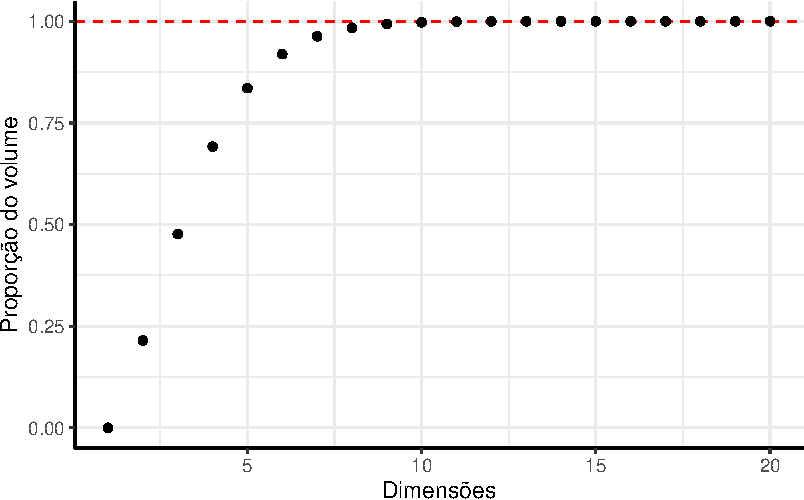
\includegraphics{lista-1_files/figure-pdf/fig-grafico-q2-1.pdf}

}

\caption{\label{fig-grafico-q2}Proporção do volume do hipercubo que está
fora da hiperesfera em função da dimensão do espaço.}

\end{figure}%

\newpage{}

\section{Referências}\label{referuxeancias}

\phantomsection\label{refs}
\begin{CSLReferences}{1}{0}
\bibitem[\citeproctext]{ref-anderlucci2019}
Anderlucci, Laura, Angela Montanari, e Cinzia Viroli. 2019. {«The
Importance of Being Clustered: Uncluttering the Trends of Statistics
from 1970 to 2015»}. \emph{Statistical Science} 34 (2).
\url{https://doi.org/10.1214/18-sts686}.

\bibitem[\citeproctext]{ref-armstrong1989}
Armstrong, Ben G., e Margaret Sloan. 1989. {«Ordinal Regression Models
for Epidemiologic Data»}. \emph{American Journal of Epidemiology} 129
(1): 191--204. \url{https://doi.org/10.1093/oxfordjournals.aje.a115109}.

\bibitem[\citeproctext]{ref-pitombo2015}
Pitombo, Cira Souza, e Aline Schindler Gomes da Costa. 2015. {«Aplicação
conjunta de modelos não paramétricos e paramétricos para previsão de
escolha modal»}. \emph{Journal of Transport Literature} 9 (1): 30--34.
\url{https://doi.org/10.1590/2238-1031.jtl.v9n1a6}.

\end{CSLReferences}



\end{document}
